\chapter{Introduction}
With this chapter, the reader should be able to comprehend why this thesis was written, 
what it tries to accomplish and which topics are considered within the scope of this work.

\section{Motivation}

The increasing amount of Platform-as-a-Service (PaaS) solutions, cloud-hosted environments and microservice architectures introduce new attack scenarios. 
This creates the need for new defense strategies in both Development and Operations. 
Especially solutions providing \gls{k8s} compliant container orchestration are identifiably different and in high demand compared to long established solutions. 
This calls for a more detailed, focused examination. 

\section{Objective}

This thesis aims to answer the following questions:

\begin{itemize}

\item What generic security risks emerge when providing or using a multi-tenant PaaS solution,
with each tenant developing, deploying and running their own applications? 

\item How can a PaaS provider (serving internal and/or external users) mitigate those risks? 

\item  In this scope and from a PaaS provider viewpoint, how does an on-premise solution compare
to a public cloud solution? 

\end{itemize}

Another goal is to recommend security measures for different implementation use cases.
A comparison of existing risks and the need for action derived from it should serve as central point of view. 
Possible measures to mitigate those risks shall be explored, evaluated and exemplary put to use in practical examples.
Subsequently the risk will be re-evaluated in order to illustrate a viable risk management method.
With the results gathered, the thesis will compare different best practice implementations for different use cases and recommend measures for each.

\section{Scope limitation}

To achieve the aforementioned goals, the thesis will first limit the view on the problem to a manageable scope by
concentrating on the components enabled by default and those required for operations of two established and \gls{k8s} compliant solutions.
These solutions will be \gls{ocp} as an on-premise solution and \gls{aks} as a public cloud solution. 
The latest stable version of \gls{ocp} during the work on this thesis was version 3.11\footcite{ocpRelease}, which is based on the \gls{okd} 3.11. \gls{okd} is a fork of \gls{k8s} 1.11.0 with additional edits and updates (refer to section \ref{openshiftExplanation} for details).
Through \gls{aks}, kubernetes v1.13.5 was already available at the same point in time. In order to better compare both implementations, the available \gls{k8s} version 1.11 was chosen for \gls{aks}.
%TODO add proof of azure version availability in appendix and reference it! (see screenshot pptx)
Components providing \gls{k8s} compliance will be the main focus, as these bear the most significance across all Kubernetes Certified solutions. 
A look at popular tools and frameworks used in such clusters will be avoided in order to keep the scope manageable, though some might be recommended as a mitigation.
In order to be applicable to a higher number of use cases, attacks and measures seen in environments with exceptionally high security requirements might be mentioned , but not  covered in their entirety. This might entail state-sponsored actors deploying zero-day exploits, which are not applicable to a majority of solutions deployed.
This thesis aims to provide insight to the risks of providing a PaaS solution and mitigations thereof. 
As such, it will look at the capabilities a potential provider has to (mis-)configure such solutions - inherent risks of the technologies themselves are only explored when measures to mitigate them are accessible from a provider standpoint. 
In short, the goal is to improve the security of your \gls{k8s} cluster, not \gls{k8s} itself.
To follow the OWASP Risk Rating Methodology\footcite{riskRating} down the line, we need to define our threat agents. It is recommended to minimize the number of threat agents by treating them as equivalent classes when applicable\footcite{threatModeling}. Examining a list of threat actors published through SANS\footcite{sansThreatActors}, we can will only exclude state-sponsored actors. This leaves us with cyber criminals, hacktivists, systems administrators, end users, executives and partners.
Grouping the remaining actors by the factors used to estimate risks in section \ref{riskEstimate}, we can identify find three scenarios that encompass all of the actors:

%TODO Mention baseline security in summary!
%TODO change summary to fit the items here!
\begin{itemize}

\item Malicious third party attacking the solution from within the \gls{lan} and/or the internet

\item Malicious third party attacking from inside a hijacked container, i.e. remotely executing code or commands

\item Bad user, i.e. a negligent, hijacked or malicious account risking compromise of their own and/or other applications

\end{itemize}

\chapter{Theory}
With this chapter, a reader with foundational knowledge of topics regarding Computer Science and/or Informatics 
should be able to grasp the specialized technologies discussed within the thesis and familiarize themselves with the definitions and terminology used throughout it.

\section{Infrastructure-as-a-Service}
In \gls{iaas} environments, a consumer trusts his \gls{iaas} provider with the management and control of the infrastructure needed to deploy his applications.
The provided service ends at provisioning of processing, storage, networks and other computing resources.\footcite{nistcloud}
Therefore consumers do not need to manage their own data centers or topics like system uplink availability.
As shown in Figure ~\ref{fig:servicecomparison}, consumers are responsible for the \gls{os} layer and everything above it.

\begin{figure}[H]
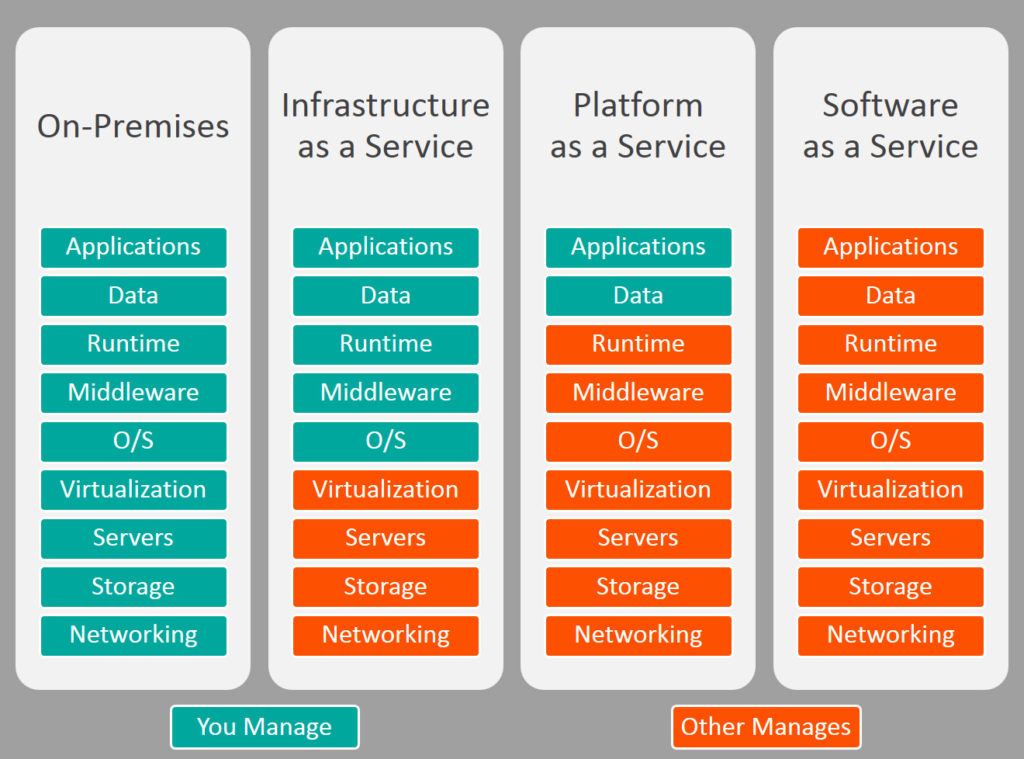
\includegraphics[scale=0.4]{pictures/ServiceComparison.jpg} 
\caption{Comparison of responsibilities in different service models\protect\footcite{servicecomparison}}
\label{fig:servicecomparison}
\end{figure}

\section{Platform-as-a-Service}

In \gls{paas} environments, a consumer trusts his \gls{paas} provider with the management and control of even more resources needed to deploy his applications beyond those covered by \gls{iaas}.\footcite{nistcloud}
In an ideal scenario, this leads to a consumer not having to concern himself with the underlying network, hardware, servers, operating systems, storage or even common middleware like log data collection and analysis\footcite{msPaas} and allows him to focus on other tasks, i.e. application development.
As a downside to this, a consumer might only have limited control on, among other factors, the software installed on the provisioned machines. 
Although this shifts some of the responsibility burden towards the provider, the situation isn't as clear-cut as one might think. 
Figure ~\ref{fig:servicecomparison} shows middleware and runtime as provided, but there is no clear standard on what capabilities or tools are included.
A consumer might require capabilities which aren't provided or wishes to avoid provider lock-in through proprietary tools, 
again resulting in middleware responsibilities for the consumer. 
A consumer might also have to extensively configure the application-hosting environment for compliance or security purposes. 
Even some low-level tasks aren't completely managed, i.e. \gls{vm} reboots to apply security updates.\footcite{msVmReboot}

\section{Containers}

In order to run and manage containers, several components and systems are needed. The most important ones will be introduced here.

\subsection{What are containers?}
As the Docker website puts it, a container is a standard unit of software that packages up code and all its dependencies so the application runs quickly and reliably from one computing environment to another.\footcite{whatContainer}
From a technical viewpoint, a container is an isolated process running in the userspace on a host \gls{os}. The host system shares the kernel with all containers on it and might share other resources, but containers are built from container images which include any code and dependencies needed in order to make them independent of the infrastructure they are running on.\footcite{containerIntro}

Linux containers were widely popularized through Docker, a container system initially based on \gls{lxc}.\footcite{containerHistory}
Containers provide isolation of multiple appllications running on the same machine and are often deployed in environments where this isolation would formerly have been achieved by using multiple \gls{vm}s, which is why they are often compared to them despite the fundamental technical differences. The Kubernetes documentation illustrates the differences as seen in Figure ~\ref{fig:VMsVsContainers}.

\begin{figure}[H]
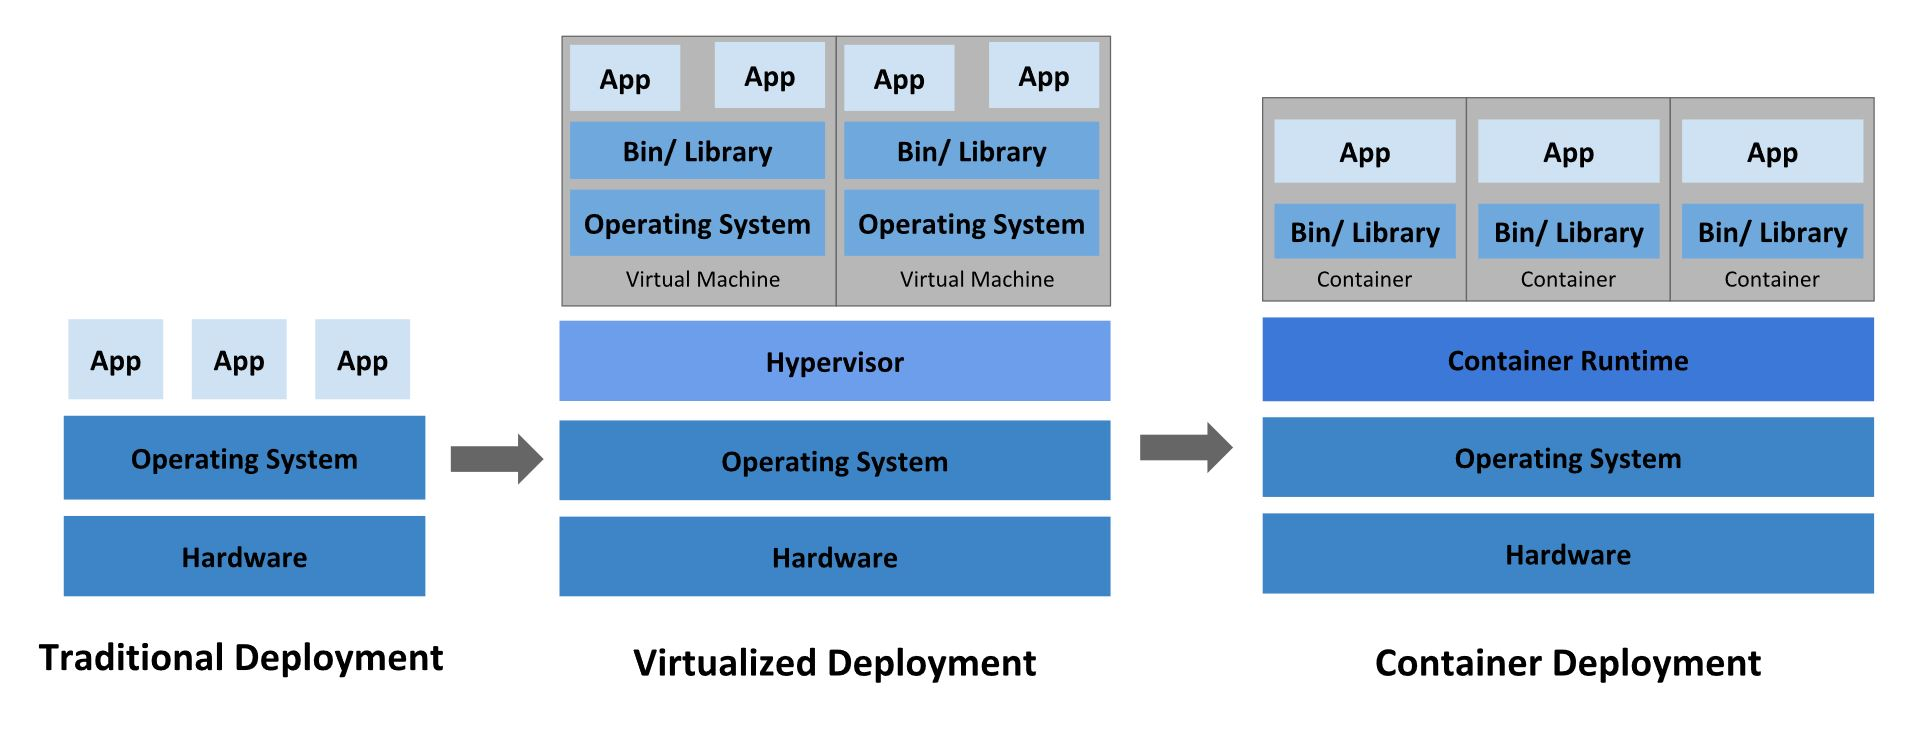
\includegraphics[scale=0.3]{pictures/VMsVsContainers.jpg} 
\caption{Comparison of different application deployments on the same hardware\protect\footcite{k8sDocsVmsContainers}}
\label{fig:VMsVsContainers}
\end{figure}

\subsection{Differentiating docker}
Talking about docker can be quite difficult, since the term refers to multiple things at once - a company (Docker Inc.), their commercial products (Docker CE and Docker EE) and the former name of their open source project (Docker, now called Moby).\footcite{dockerMoby}
Additionally, there is a \gls{cli} called docker engine, which serves as an interface to the containers running on a host. It includes a high-level container runtime (which will be talked about in the following section).\footcite{dockerEngine}
Some sources also talk about docker-formatted containers if those implement the same interfaces as the docker container runtime.\footcite{dockerFormatted}

\subsection{Images, image building and Dockerfiles}
A container image is a binary including all the data needed to run a container. It might also contain metadata on its needs and capabilities, i.e. version information through tags.\footcite{redhatImages}
Container images are sometimes referred to as docker images or docker-formatted images, but they can be run by other container runtimes and vice-versa.
In order to create a container image, you have to build it. This is often done through a build process executed by a container runtime. The instructions for container builds are commonly defined and documented in a Dockerfile\footcite{dockerfileDocs} (which may also be done by non-docker programs, adding onto the vocabulary confusion).
Container images can be distributed through container image registries, where images can be uploaded to and downloaded from. A commonly known example is docker hub, a public registry run by Docker Inc.

\subsection{Container standards and interfaces}

Without going into the nuances and historical developments, there are a multitude of programs mostly implementing three interfaces for container management.
The two basic interfaces are the runtime and image specifications under the \gls{oci} which standardize how containers and container images should be formatted and executed.\footcite{ociStandards}
The \gls{oci} also maintains a reference implementation called runc, alternatives include rkt and lmctfy.\footcite{lowLevelRuntimes}
Runc and similar programs implementing these specifications are commonly called low level runtimes, in contrast to the high level runtimes that control them.
These high level runtimes like containerd or CRI-O commonly manage more abstract features like downloading and verifying container images.\footcite{highLevelRuntimes}
Many high level runtimes today adhere to the \gls{cri} so they can be used interchangeably by container orchestrators.\footcite{criDocs}

%TODO maybe shorten and just talk about CRI upwards?

\section{Container Orchestration}
Once you want to use multiple containers on different machines talking to each other and offering stable services that continue even when some containers fail, the need for automated systems to manage these containers arises. Orchestrators can also provide many other advantages, like load balancing and automated scaling.
Kubernetes systems are the most prevalent orchestrators currently in use.
%TODO citation for kubernetes market share?

%TODO
idea: control system, architecture (control plane vs. application(s), kubelet, master/non-master nodes, ...), standard (can have other implementations), certification requirements, uses in general and in \gls{aks} and \gls{ocp} specifically.

\subsection{Kubernetes}
LINKS COMMENTED

%https://kubernetes.io/docs/concepts/\#overview \\
%https://kubernetes.io/docs/concepts/overview/components/ \\
%https://res.cloudinary.com/dukp6c7f7/image/upload/f\_auto,fl\_lossy,q\_auto/s3-ghost/2016/06/o7leok.png \\

\subsubsection{Kubernetes Objects}
TODO
higher-level idea behind objects
Pods, Services, Volumes, Namespaces

\subsubsection{Kubernetes Controllers}
TODO

higher-level idea behind controllers
ReplicaSets, Deployments, StatefulSets, DaemonSets, Jobs

\subsubsection{Using Kubernetes}
TODO

build from scratch, buy CaaS/PaaS/IaaS, cloud vs. on-prem, different scopes/features from different products

https://kubernetes.io/docs/setup/pick-right-solution/

\subsection{OpenShift} \label{openshiftExplanation}
TODO
%TODO OCP-> OKD -> k8s, mention that security fixes of k8s upstream are applied!

\subsection{Azure Kubernetes Service}
TODO

\section{TODO: Others?}
TODO

\chapter{Deriving the attack surface}

\section{Defining procedure and approach}

%TODO: derive all 20 vectors from the three scenarios, explain why you cannot prove that this is/will be everything, explain why grouped this way \& which systems/threat actors rolled together in it. List security measures for each.


\section{Identified vectors}
%TODO: write out pretty

\subsection{Reconaissance through Kubernetes and platform control plane interfaces}
Gather information useful for further attacks through accessible: the Kubernetes dashboard \& apiserver as well as potential platform webinterfaces \& apiserver(s)

components: kubernetes dashboard, kubernetes apiserver, OCP web console, 

TODO

\subsection{Read confidentials through Kubernetes control plane interfaces}
Gather confidential information through the Kubernetes dashboard \& apiserver (platform interfaces are evaluated separately)
TODO

\subsection{Change configuration through Kubernetes control plane interfaces}
Change the existing configuration through the Kubernetes dashboard \& apiserver (platform interfaces are evaluated separately)
TODO

\subsection{Read confidentials through platform interfaces (mgmt console/API)}
Gather confidential information through platform webinterfaces \& apiserver(s) (Kubernetes interfaces are evaluated separately)
TODO

\subsection{Change configuration through platform interfaces (mgmt console/API)}
Change the existing configuration through platform webinterfaces \& apiserver(s) (Kubernetes interfaces are evaluated separately)
TODO

\subsection{Compromise internal k8s control plane components (etcd, scheduler, controller-manager)}
This vector comprises reconaissance, leaks of confidentials and configuration changes through Kubernetes components not intended to be accessible: etcd stores, kube-scheduler and kube-controller-manager
TODO

\subsection{Supply compromised container (base) image}
Supplying a malicious container image leading to security violations on the cluster (remote access for an attacker, resource misuse, data leakage, …). Most easily done untargeted (dockerhub images or dockerfiles on tutorials/help forums), but can be done targeted, too. Additionally, an image build process typically runs as root, leading to compromise possibilities to compromise the node where an image is built from a rogue dockerfile. (TODO: provoking stale image usage to exploit vulns, too?)
TODO

\subsection{Supply compromised k8s configuration}
Supplying a malicious kubernetes configuration leading to security violations on the cluster (remote access for an attacker, resource misuse, data leakage, …). Most easily done untargeted (tutorials/ help forums), but can be done targeted, too.
TODO

\subsection{Compromise other application components (lateral movement)}
Once an attacker gains access to a container, he may try to access more lucrative application components or information, i.e. sniffing traffic or accessing databases or containers with more confidential information/traffic.
TODO

\subsection{Container breakout (R/W, Privilege Escalation)}
Once inside a container, an attacker may try to gain access to the underlying host by a multitude of means. This includes invoking syscalls, accessing the host file system and elevation priviledges within or outside of the container environment
TODO

\subsection{Compromise local image cache}
If the cached image of a container can be manipulated, another container (which might even seem to fulfill the same function) violating security principles could be started.
TODO

\subsection{Modify running container}
Once inside a container, an attacker may try to modify the container to exfiltrate data or better suit their needs for further intrusion
TODO

\subsection{Misuse node resources (sabotage, cryptojacking)}
The resources of a single node are used to run a container and may be misconfigured or misused for financial gains (mining cryptocurrencies) or to disrupt service availability (i.e. through fork bombing or misconfiguration)
TODO

\subsection{Hoard orchestration resources (sabotage)}
The resources of the whole cluster may be misconfigured or misused to disrupt service availability (i.e. through fork bombing or misconfiguration)
TODO

\subsection{Misuse orchestration resources (cryptojacking)}
The resources of the whole cluster may be misconfigured or misused for financial gains (mining cryptocurrencies)
TODO

\subsection{Add malicious container}
A malicious container may be started within the cluster
TODO

\subsection{Add malicious node}
A malicious node may be added to the cluster
TODO

\subsection{Bad user practice (outside of cluster)}
This vector comprises user practices outside of the cluster that lead to risks within it. Examples include phishing, openly publishing keys/tokens to public code repositories and more.
TODO

%TODO: dont forget
%default kubeconfig file location on user machine: $HOME/.kube/config <- contains certs + tokens for login, specifies which apiservers, ...
%get token from user: oc whoami --token
% call API with user token:	curl -X GET -H "Authorization: Bearer <token>" https://openshift.redhat.com:8443/oapi/v1 --insecure %
% login with user token:	oc login --token '<token>'
% check user rights: 

\subsection{Incufficient base infrastructure hardening}
The underlying nodes could allow an attacker easy entry, even if the containers themselves are hardened
%TODO: also other (external) parts of company infrastructure
TODO

\subsection{Entry through known, unpatched vulnerabilities}
Every system has to be kept up to date with  security patches. Publicly known vulnerabilities might otherwise be exploited, leading to potentially devastating violations of security principles
TODO


\chapter{Assessing the attack surface risk}
%TODO: derive process/evolution of risk rating model, introduce rating by threat actors + tools + vector + platform, explain problems / inaccuracies%

\section{Defining procedures and approach}

In order to achieve a view on the risks more accurately resembling situations where a solution might be implemented, several assumptions are made:

\begin{itemize}

\item People in contact with the solution are familiar with conventional security principles and measures, but are new to the technologies used in the solutions within scope. They might even be new to container and cloud solutions in general. This includes both users of the solution like developers and project managers, as well as operators and administrators.

\item It is assumed that no special requirements like industry-specific compliance requirements have to be followed and the workloads processed within the solution have no exceptionally high security requirements. 

\item Regarding the design and implementation of applications running on the solutions, it is assumed that conventional application security measures have been implemented, i.e. against the OWASP Top 10.\footcite{topten} The extent of those measures is assumed to be in accordance to moderate criticality of the data and service provided by the application.

\item Some risks increase or decrease drastically, depending on many specific configurations. Considering the high system complexity, ``getting it to work'' is hard enough for users and operators new to these technologies.\footcite{hackAndHarden} When setting up and configuring a setup, the default configurations are left as-is whenever possible. Guidelines of specific implementations are followed, but whenever measures are presented as optional and not required, they will be skipped. Before recommending security measures, the setup will be modified just enough to become functional, without regards to the security implementations.

\item Multiple tenants like different customers, teams or projects are separated by \gls{k8s} namespaces or \gls{ocp} projects respectively, not by clusters.

\end{itemize}


%START OLD STUFF, REVISIT%
Focus on three scenarios: attack through network, hijacked container, bad user

Research-Freeze: May 3rd, 2019! (Pre-KubeCon19, check git commit dates for stuff like OWASP-documents etc!)
Some newer information might be used for big outliers, but everything else just gets a side note

RISK ASSESSMENT METHODOLOGY:
difficulties with: 
A how generically should vectors be set?
B how to structure vectors (into categories?) 

Solution to A: vectors split and merged after risk assessment sketch; if there were considerable differences in the estimated values, they were split. If no diffs, they were merged.
Solution to B: Considerable time invested, no optimal solution was found. Ultimately ignored this, since more time investment wasnt feasible or added much value to the goals. TODO: Explain process, what was looked at and why it wasnt good, how we arrived at the end structure.

Risk assessment formula:
Risk = Probability * Impact.
Impact was taken as single value of 1 through 3  and estimated through None/Theoretical (0), Low/Intermediate-Step (1), non-severe security principle violation (2), severe security principle violation (3)

Probability was a bitch to define proberly. Therefore split into four factors: Vantage Point, Required Access Level (RAL), Detectability and Exploitability. Those initially had values between 0 though 3, but outlier values of 4  were defined for RAL and Vantage Point (in sync with existing assessment methodologies within HvS).
The average of these four values is taken as the total propability value, ranging from 0.25 through 3.5 (low <= 1.25, medium <= 2.25).
Vantage Point: physical access (0, see above since your own or the cloud providers hardware-accessing employees can also do whatever they want); node or management-interface (1); within container (2); within company network (3); from public www (4)
Required Access Level: cloud/infrastructure admin (0, since a rogue employee with super-admin can do whatever they want and this is about baseline security); cluster/system-admin (1); cluster/system user with read/write access (2); cluster/system user with read-only access (3); unauthenticated (4)
Detectability: Difficult (1) since it needs custom tools for environment-specific vuln detction; Average (2) since it is either generic but needs simple custom tools or its individualized but can be identified with some slight tool individualization; Easy (3) since there are generic script-kiddie tools / GUI-paths to find the vuln
Exploitability: Theoretical (0, since this is the level of unpublished 0-days and we are still doing baseline security); difficult (1) needs custom tools for environment-specific exploitation; Average(2), since its a generic exploit but needs simple custom tools or its inividualized but can be exploited with some slight tool individualization; Easy (3) since there are generic script-kiddie tools / GUI-paths to exploit the vuln

This leads to a total risk of 0 through 10.5, which is then rounded to full integers and capped at 10. In accordance to HvS internal models, total risk values <= 3 are defined as low, <= 6 as medium and values above that are defined as high.

specific values for each vector are estimated in a context with multiple assumptions:
TODO: callback to assumptions in scope limitation

- If multiple techniques can be used / impacts can occur to leverage a vector, all factor values of the one with the highest total risk are taken
- Values might decrease through the implementation of security measures, leading to a lower total value. (If multiple techniques could be used to leverage a vector and only one gets its total risk reduced, the new maximum risk value of that vector becomes the vector value(s)

goal is to reduce values above threshold X to below threshold X by applying security measures. This aims to ensure a basic security level, not something against APT groups / zero-day protection / targeted attacks with a lot of resources and competence. (no online banking, user data of average confidentiality etc)

Default values are defined as the following:

SETUP OF PRACTICAL PART:

Version freeze:
\gls{ocp} 3.11 -> OKD 3.11 ->  k8s-version = 1.11(.0 with fixes, is a fork. see: https://github.com/openshift/origin/releases/tag/v3.11.0 )
AKS (on May 3rd 2019) => k8s-version <= v1.13.5 available, but only for k8s-v1.11 only 1.11.8 or 1.11.9!

Considerable changes between 1.11.0 and 1.11.9 (Source: https://github.com/kubernetes/kubernetes/blob/master/CHANGELOG-1.11.md):
- action required: the API server and client-go libraries have been fixed to support additional non-alpha-numeric characters in UserInfo "extra" data keys. Both should be updated in order to properly support extra data containing "/" characters or other characters disallowed in HTTP headers. (\#65799, @dekkagaijin)
- https://github.com/kubernetes/autoscaler/releases/tag/cluster-autoscaler-1.3.1
- ACTION REQUIRED: Removes defaulting of CSI file system type to ext4. All the production drivers listed under https://kubernetes-csi.github.io/docs/Drivers.html were inspected and should not be impacted after this change. If you are using a driver not in that list, please test the drivers on an updated test cluster first. ``` (\#65499, @krunaljain)
- kube-apiserver: the Priority admission plugin is now enabled by default when using --enable-admission-plugins. If using --admission-control to fully specify the set of admission plugins, the Priority admission plugin should be added if using the PodPriority feature, which is enabled by default in 1.11. (\#65739, @liggitt)
The system-node-critical and system-cluster-critical priority classes are now limited to the kube-system namespace by the PodPriority admission plugin. (\#65593, @bsalamat)

no major changes => OCP 3.11, AKS-k8s 1.11.9!

Dependency compatibilities:
OCP 3.11: docker 1.13, CRI-O 1.11 (Source: LINK COMMENTED %https://docs.openshift.com/container-platform/3.11/release_notes/ocp_3_11_release_notes.html#ocp-311-about-this-release)
k8s-1.11: docker 1.11.2 to 1.13.1  (Source: LINK COMMENTED % https://github.com/kubernetes/kubernetes/blob/master/CHANGELOG-1.11.md#external-dependencies), CRI-O 1.11 (in-synch to k8s releases, source: https://github.com/cri-o/cri-o)
Azure-AKS: uses moby, NOT docker! (moby = pluggable container runtime based on docker, automatically updated in background whenever no node restart needed)

-> take defaults for all dependencies on install, document and apply all AKS node updates needing manual restart!
TODO: apply OCP updates when incoming?

%TODO: END OLD STUFF, REVISIT%

\section{Estimating the risk} \label{riskEstimate}
%TODO: derive \& explain values for each vector

\subsection{Reconaissance through Kubernetes \& platform control plane interfaces}

%OCP
A user with access to the apiserver / webinterface(s) and read access can scout out information.
By default, each account (project admin or project user, but not cluster admin) can only see information about his own project, a cluster admin can see all namespaces.
This could show outdated software versions, running systems / containers / pods / user account privileges / misconfigurations and may support in planning and confirming effectiveness of further attacks.

The information gathering processes and interfaces are known and documented pretty well, but the information gathered has to be analyzed specific to the environment.
%AKS
Same as OCP, except accessible from anywhere (cloud, duh).
-> doesn’t change total risk value

\subsection{Read confidentials through Kubernetes control plane interfaces}
%OCP
In addition to V01, a user with access to the apiserver / webinterface(s) and read access can gather confidential secrets like certs, tokens or passwords which are intended to be used by automated systems and/or users to authenticate themselves to cluster components and gain privileged access like pull/push images, trigger actions in other applications / containers, …
These can be gathered and used for further access by an attacker.

Kube-hunter is a readily available tool and checks for this automatically.

%AKS
Same as OCP, except accessible from anywhere (cloud, duh).
-> increases total risk value slightly, pushing it just over the edge from medium to high

\subsection{Change configuration through Kubernetes control plane interfaces}
%OCP
In adition to both V01 and V02, a user with access to the apiserver / webinterface(s) and write access can change configurations on the cluster. By default, each account (project admin or project user, but not cluster admin) can only change the configuration of namespaces resources (i.e. access to project-specific resources like pods, services, routes, but not cluster-global resources like nodes, SCCs or interface/authorization configurations). 

The capabilities can be looked up through the API, what you can achieve with it has to be analyzed environment-specifically though.

%AKS
Same as OCP, except accessible from anywhere (cloud, duh).
-> increases total risk value slightly, both are still rated high in the end

\subsection{Read confidentials through platform interfaces (mgmt console/API)}
%OCP
Same as V02, TODO: merge

%AKS
Same as V02, TODO: merge

\subsection{Change configuration through platform interfaces (mgmt console/API)}
%OCP
Same as V03, TODO: merge

%AKS
Same as V03, TODO: merge

\subsection{Compromise internal k8s control plane components (etcd, scheduler, controller-manager)}
%OCP
Misconfiguration of internal Kubernetes components (accessible by systems it is not assigned to be accessible by) could lead to a full cluster compromise. The cluster configuration and all secrets / authorization credentials are stored in the etcd instance(s). One would need to seriously fuck up the setup, since OCP configures everything through ansible and you would have to knowingly change some internal settings not intended to be changed in order to achieve this. Configurations are maintained by red hat, meaning config changes will be applied in updates and additionally sent out to notify relevant people subscribed to those alerts.

Kube-hunter checks for misconfiguration, but can’t find any (non-false-positive) openings with default settings. Would need zero-day / known vuln in Microsoft or red hat configs

%AKS
Same as OCP, except accessible from anywhere (cloud, duh).
The master components are updated, configured and maintained by Microsoft, only when a restart is required the cluster administrator has to trigger it manually.
-> increases total risk value slightly, both are still rated medium in the end

\subsection{Supply compromised container (base) image}
%OCP
This has two facettes: it can be untargeted (image spraying) and targeted (compromising a specific image known to be used by the target).

The untargeted version needs the least access, since it simply needs a (free) dockerhub account to upload malicious images that could or couldn’t fulfil the function they are advertised to do. This is done in the hopes of someone downloading that image for use in his own environment, thus starting attacker-supplied containers within their cluster.
This could allow an attacker remote access to a container in the cluster and/or exfiltrate information.
Even without injecting malware, an attacker could mislabel old software versions as newer ones so software with known vulnerabilities is deployed because it is though to be up to date.

The targeted version could be specialized uploads to docker hub (similar to broad phishing vs. spear phishing) or “poisoning” an internal container image repository.

Image builds run as root, which could further be exploited – but this would need a vulnerability in the OCP / Azure build process.

These methods are publically known and both the docker container runtime and docker hub actively try to mitigate this, but malicious images are only deleted when reported by enough users and the security settings within the container runtime are not set by default.
Base containers and malware / known vulnerable versions are readily available from public sources, but need some technical expertise to plug together.

%AKS
Exactly the same as OCP

\subsection{Supply compromised k8s configuration}
%OCP
Similar to V07, this can be done either untargeted by spraying to tutorials / help forums or targeted, similar to spear phising.
If a cluster administrator does not fully analyze or understand the configuration he gets from public sources, the cluster could be compromised fully, i.e. by implementing backdoors through malicious containers with special access and ability to be remotely accessed by the attacker.

Examples are readily available from public sources, but need some technical expertise to plug together.

%AKS
Exactly the same as OCP

\subsection{Compromise other application components (lateral movement)}
%OCP
Once an attacker sits within a container, he can scan the network for other containers, hosts, services, apis or similar interfaces to further his access. By default, all containers in all projects (except master \& infra components) are put in the same subnet, allowing everyone to communicate with anyone else.
This is especially troubling for securing an environment with multiple tenants – even if the DB is not publically accessible, unauthorized access can be leveraged by anyone in the cluster.

Scanning tools like nmap etc. to find components to talk to are readily available, but their results are cluster-specific (everyone runs something different). Therefore some technical expertise is needed to leverage the network access needed. 

%AKS
Same as OCP. 
The worst AKS-specific problem with this is the mitigation. This risk is not clearly documented in the setup section of the documentation. If one stumbles upon this information in further sections of the docs after setting up his cluster, he might postpone or deny changing the setting to isolate different projects by default. This is because a full cluster rebuild is needed to change this setting!

\subsection{Container breakout (R/W, Privilege Escalation)}
%OCP
A deployed container poses the risk of allowing access to the node it is running on, thus allowing an attacker to “break out” of the container and perform actions on the node.
This poses a considerable threat, since any container may run on any node by default, allowing an attacker full access to any containers running on the node he controls, which will – especially over time – have a great chance to include containers belonging to other projects.

The OCP default settings limit the possibility of this dramatically, the risk lies more in organizations relaxing the defaults in favour of easy usability. (A majority of container images straight from docker hub require UID 0, which is denied by the default SCC ‘restricted’ in OCP during admission. This results in crashlooping and non-functional containers, developers would need to customize any image themselves. The easiest way to stop those problems this is to permit the default service account within a project access to the ‘privileged’ SCC permissions. This would significantly increase the risk of a container breakout!)

This is probably the most-talked about attack vector regarding containers, but techniques are not obviously documented and breakout methods would have to be customized to the restrictions applied within a cluster.

%AKS
Difference to OCP: containers can be run with UID 0 and more relaxed settings in general by default. User-namespace remapping not in place by default, vastly increasing the risk of a container breakout!
This is more on the usability>security side of things. 
-> raises risk, jumping from medium to high.


\subsection{Compromise local image cache}
%OCP
If you can swap out the cached container image on a host, the swapped-in version will run the next time this node spins up this container.
This is a very sneaky way to inject a malicious container, but within the default settings, access to the host file system is required.

Not well known and not entirely trivial to do (sneakily).

%AKS
Same as OCP.

\subsection{Modify running container}
%OCP
Instead of deploying a container with malicious contents, an attacker can try to modify and use an already running container to its needs by loading additional tools/binaries, changing configurations or exfiltrating data. This could be done through an RCE vuln, ssh access or others, just like any compromised linux machine.

-> Common sense to do this, same technical level as any command line interaction with a linux system.

%AKS
Same as OCP.

\subsection{Misuse node resources (sabotage, cryptojacking)}
%OCP
This is a vector in contrast to orchestration resources.
Assuming a cluster suitable for production (more than one worker node, probably more than a handful), the failure or misuse of a single node may be of use to the attacker, but has very limited impact to operations. This is because a significant part of the cluster is built to heal from failures of any node and/or container.
TODO: absorb this with V14 and V15, since the risk is always lower than them and they cover everything?

Mining containers/binaries and/or fork-bombing tools with accompanying tutorials are easy to find publically. Cryptojacking is regularly cited as an up-and-coming attack.

%AKS
Same as OCP.

\subsection{Hoard orchestration resources (sabotage)}
%OCP
With enough access or restrictions too lax, an attacker may be able to seriously halt the availability of all workloads processed by the cluster by misconfiguration, conducting DOS attacks or wiping nodes or cluster configurations. Since it is a complex system, finding the sabotaged component can take considerable know-how and time if done well, increasing the impact – especially in on-premise environments, where resources are limited.

Wiping is common sense, sabotaging the cluster in a complex and effective way may take deeper knowledge and be customized to the environment.

%AKS
Difference to OCP: you can easily spin up more resources in the cloud -> less impact
-> risk decreases by a considerable margin, high to medium

\subsection{Misuse orchestration resources (cryptojacking)}
%OCP
In contrast to V14, an attacker will try to be sneaky if done well.
The goal here is to (ab)use the computing resources not belonging to and payed for by him to achieve monetary gain though mining cryptocurrencies.

Cryptojacking is regularly cited as an up-and-coming attack, but to do it with a low risk of being detected needs some technical skill.

%AKS
Difference to OCP: an attacker can easily spin up more resources in the cloud -> more impact
-> risk increases by a considerable margin, medium to high

\subsection{Add malicious container}
%OCP
Instead of manipulating running containers, an attacker with user access and permissions to spin up containers may start their own ones. (BYOC – bring-your-own-container?)
This is still restricted by container admission restrictions on the user/project, but at least he can install all needed binaries beforehand and his shell doesn’t die whenever the underlying container might be stopped.

Doing this is common sense, as before some technical skill is required to prepare a malicious container

%AKS
Same as OCP, except accessible from anywhere (cloud, duh).
-> increases total risk value slightly, both are still rated medium in the end

\subsection{Add malicious node}
%OCP
An attacker could try to add a malicious node to the cluster and inspect or manipulate data in or exfiltrate data from containers scheduled on it. Since any container may run anywhere, there is a high chance of all containers eventually being run on a given node over time, exposing the whole cluster to an attacker. This could be sped up by manipulating the reports of remaining resources on the node towards the scheduler.
By design, cluster administrator access is needed to add a node within OCP.

This technique is not talked about that much, but still available in public resources and possible in all clusters. Docs are publically available to add nodes to a cluster, basic linux server administration skills are needed to follow them.

%AKS
Accessible from anywhere (cloud).
-> total risk value unchanged
In contrast to OCP, you can spin up additional nodes more easily in AKS if configured on creation, but to access/control/manipulate them you still need cluster administrator access.
A tutorial on getting ssh access is available, but that’s lengthy and not trivial.

\subsection{Bad user practice (outside of cluster)}
%OCP
This vector comprises user practices outside of the cluster that lead to risks within it. Examples include phishing, openly publishing keys/tokens to public code repositories, password reuse, scouting specific software or container images used, publishing logs with information valuable to an attacker and more.
Could be done targeted (i.e. specific OSINT) or untargeted through github crawlers, scanning account/password dumps, …
Whatever you get could be used to access the cluster with the permissions granted by service-/user-accounts or as a reconnaissance base for further attacks.

There are tools available to do this, using them effectively requires some technical skill.

%AKS
Same as OCP, except accessible from anywhere (cloud, duh).
-> doesn’t change total risk value

\subsection{Incufficient base infrastructure hardening}
%OCP
The underlying nodes could allow an attacker easy entry, even if the containers themselves are hardened. This includes Side-Channel attacks like Spectre \& Meltdown, open ports on the servers exposed by other stuff running on it, being available from the public www, …
Vector exists mostly to sink all “classic” infra security measures in it, since those are researched and available everywhere and very much not the focus of the thesis.

Among worst case: unauthenticated access to run commands which is hosted publically on the internet for anyone to access and indexed by shodan. Bye bye cluster.
(Too many scenarios to hypothesize here, I’ll just point the finger at conventional server \& infra hardening standards and guidelines)

-> Well known, still needs some technical skill to find vulns and exploit them

%AKS
Suprisingly, same as OCP (despite the azure promise of PaaS-we-manage-your-infra)!
That’s the case since security updates on nodes that require a reboot are not done automatically, but have to be triggered manually or configured to trigger automatically.
Remediation is far less work though.

\subsection{Entry through known, unpatched vulnerabilities}
%OCP
Sinkhole vector for patch management. Would be a measure against every preceding vector otherwise.
Worst case could be anything, thus maximum risk. (See kubernetes CVE with 9.8 / 10)

To check for this is common sense, some technical skill may be needed to find and exploit unpatched stuff.

%AKS
Same as OCP. Even infra still needs user interaction to be patched, see preceding vector.

\chapter{Managing the attack surface risk}

\section{Defining procedures and approach}
%TODO: explain what to do if doing everything, will only implement two examples (maybe list all measures and post-measure risks in annex?)%

\section{Managing the risk of V20 - Entry through known, unpatched vulnerabilities}
%TODO: write out all from ppt with commands, pictures

\subsection{Demonstrating the successful attack without security measures}

\subsection{Selecting security measures}

\subsection{Demonstration with implemented security measures}
%TODO: maybe show again without privileged, but with uid 0?

\subsection{Risk reassessment}

\section{Managing the risk of V10 - Container Breakout}
%TODO: write out all from ppt with commands, pictures

\subsection{Demonstrating the successful attack without security measures}

%see file container_breakout.yaml!%

\subsection{Selecting security measures}

\subsection{Demonstration with implemented security measures}

\subsection{Risk reassessment}

\section{Managing the risk of V09 - lateral movement}

\subsection{Demonstrating the successful attack without security measures}

\subsection{Selecting security measures}

\subsection{Demonstration with implemented security measures}

\subsection{Risk reassessment}

\section{How to proceed}
%process only partially completed, how to proceed if you do everything. (point to completed list of measure recommendations + new risk?)

\chapter{Conclusion}

\subsection{On-premise and public cloud environment comparison}
%TODO: Comments on onPrem vs. cloud


\subsection{Multi-tenant isolation}
%TODO: Comments on multi-tenant usage
%TODO: keep this in? not a well-defined question in the beginning

\subsection{Summary}
%with outlook to future?%

% rootless container runtime \& build: https://github.com/moby/moby/pull/38050 %

